\documentclass[11pt]{exam}

\usepackage{amssymb, amsmath, amsthm, mathrsfs, multicol, graphicx} 
\usepackage{tikz}

 \def\d{\displaystyle}
\def\?{\reflectbox{?}}
\def\b#1{\mathbf{#1}}
\def\f#1{\mathfrak #1}
\def\c#1{\mathcal #1}
\def\s#1{\mathscr #1}
\def\r#1{\mathrm{#1}}
\def\N{\mathbb N}
\def\Z{\mathbb Z}
\def\Q{\mathbb Q}
\def\R{\mathbb R}
\def\C{\mathbb C}
\def\F{\mathbb F}
\def\A{\mathbb A}
\def\X{\mathbb X}
\def\E{\mathbb E}
\def\O{\mathbb O}
\def\U{\mathcal U}
\def\pow{\mathcal P}
\def\inv{^{-1}}
\def\nrml{\triangleleft}
\def\st{:}
\def\~{\widetilde}
\def\rem{\mathcal R}
\def\sigalg{$\sigma$-algebra }
\def\Gal{\mbox{Gal}}
\def\iff{\leftrightarrow}
\def\Iff{\Leftrightarrow}
\def\land{\wedge}
\def\And{\bigwedge}
\def\AAnd{\d\bigwedge\mkern-18mu\bigwedge}
\def\Vee{\bigvee}
\def\VVee{\d\Vee\mkern-18mu\Vee}
\def\imp{\rightarrow}
\def\Imp{\Rightarrow}
\def\Fi{\Leftarrow}

%\def\={\equiv}
\def\var{\mbox{var}}
\def\mod{\mbox{Mod}}
\def\Th{\mbox{Th}}
\def\sat{\mbox{Sat}}
\def\con{\mbox{Con}}
\def\bmodels{=\joinrel\mathrel|}
\def\iffmodels{\bmodels\models}
\def\dbland{\bigwedge \!\!\bigwedge}
\def\dom{\mbox{dom}}
\def\rng{\mbox{range}}
\DeclareMathOperator{\wgt}{wgt}


\def\bar{\overline}


\newcommand{\vtx}[2]{node[fill,circle,inner sep=0pt, minimum size=4pt,label=#1:#2]{}}
\newcommand{\va}[1]{\vtx{above}{#1}}
\newcommand{\vb}[1]{\vtx{below}{#1}}
\newcommand{\vr}[1]{\vtx{right}{#1}}
\newcommand{\vl}[1]{\vtx{left}{#1}}
\renewcommand{\v}{\vtx{above}{}}

\def\circleA{(-.5,0) circle (1)}
\def\circleAlabel{(-1.5,.6) node[above]{$A$}}
\def\circleB{(.5,0) circle (1)}
\def\circleBlabel{(1.5,.6) node[above]{$B$}}
\def\circleC{(0,-1) circle (1)}
\def\circleClabel{(.5,-2) node[right]{$C$}}
\def\twosetbox{(-2,-1.4) rectangle (2,1.4)}
\def\threesetbox{(-2.5,-2.4) rectangle (2.5,1.4)}
\newcommand{\twoline}[2]{\begin{pmatrix}#1 \\ #2 \end{pmatrix}}


\renewcommand{\qedsymbol}{\textsc{qed}}

%\pointname{pts}
\pointsinmargin
\marginpointname{pts}
\addpoints
\pagestyle{head}
%\printanswers

\firstpageheader{Math 228}{\bf Homework 9}{Due: Wednesday, April 8}


\begin{document}
\noindent \textbf{Instructions}: Same rules as usual - turn in your work on separate sheets of paper.  You must justify all your answers for full credit.

\begin{questions}
\question[9] Suppose that you would like to prove the following implication: 
\begin{center}
``For all numbers $n$, if $n$ is prime then $n$ is solitary". 
\end{center}
Write out the beginning and end of the argument if you were to prove the statement, 
\begin{parts}
\part Directly
\begin{solution}
To solve the above statement using a direct proof we would need to start by  assuming that $n$ is a prime number then using logic, logic, logic,... we could conclude that $n$ is solitary.
\end{solution}
\part By contrapositive
\begin{solution}
To solve by contrapositive: Assume $n$ is not solitary (logic, logic, logic...) and conclude that $n$ is not prime.
\end{solution}
\part By contradiction
\begin{solution}
To solve using a proof by contradiction: Assume that $n$ is prime and that $n$ is not solitary (logic, logic, logic...) then either $n$ is not prime or $n$ is solitary (you need to contradict one of your assumptions). Therefore, if $n$ is prime then $n$ is solitary.
\end{solution}
\end{parts}
You do not need to provide details for the proofs (since you do not know what solitary means). However, make sure that you provide the first few and last few lines of the proofs so that we can see that logical structure you would follow.



\question[9] A standard deck of 52 cards consists of 4 suites (hearts, diamonds, spades and clubs) each containing 13 different values (Ace, 2, 3, \ldots, 10, J, Q, K).  If you draw some number of cards at random you might or might not have a pair (two cards with the same value) or three cards all of the same suit.  However, if you draw enough cards, you will be guaranteed to have these.  For each of the following, find the smallest number of cards you would need to draw to be guaranteed having the specified cards.  Prove your answers.
\begin{parts}
\part Three of a kind (for example, three 7's).
\begin{solution}
The worst case scenario that could happen before you drew three of a kind would be $26$ because that would mean that you have drawn exactly $2$ of each card, Ace through King. Thus, as soon as you draw the $27$th card, you will have three of a kind.
\end{solution}
\part A flush of five cards (for example, five hearts). 
\begin{solution}
Okay, let's think about the worst case scenario again. If I drew 4 of every suit (hearts, spades, diamonds, and clubs) then I would have 16 cards and not yet have a 5 card flush. However, as soon as I draw the $17$th card, I have 5 cards of the same suit no matter which suit I draw.
\end{solution}
\part Three cards that are either all the same suit or all different suits.
\begin{solution}
You must pick 5 cards.  If you picked just 4, you could have two hearts and two spades.  However, given any 5 cards, we can be sure that at least two of them will be the same suit, say hearts.  Of the remaining three cards, if any of them are also a heart, we will have three hearts.  If not,  there are two cases to consider.  Either all three cards will be of the same suit (in which case we would have three cards of the same suit) or else two suits will be present among the three cards.  But those two other suits are not hearts, so those two cards plus one of the hearts will form a set of three cards of all different suits. 
\end{solution}
\end{parts}



\question[6] Suppose you are at a party with 19 of your closest friends (so including you, there are 20 people there).  Explain why there must be least two people at the party who are friends with the same number of people at the party.  Assume friendship is always reciprocated.

\begin{solution}
  Suppose this was not the case.  That is, suppose everyone at the party had a {\em different} number of friends.  What could these numbers be.  The would have to be less than 20, so each number from 0 to 19 (that's 20 numbers) must be used exactly once.  But this is impossible. If someone is friends with 19 people, then she is friends with everyone, including the person who is supposedly friends with 0 people.
  
  What this says is that in any simple graph with 20 vertices, there must be at least two vertices which have the same degree.
\end{solution}


\question[6] Suppose you have an $n\times n$ chessboard but your dog has eaten one of the corner squares. Can you still cover the remaining squares with dominoes? What needs to be true about $n$? Give necessary and sufficient conditions (that is, say exactly which values of $n$ work and which do not work). Prove your answers.

\begin{center}
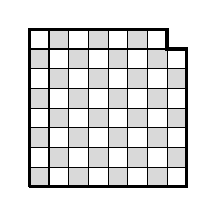
\begin{tikzpicture}[scale=.25]
\foreach \x in {0,2,...,6}{
	\foreach \y in {0,2,...,6}{
\draw[fill=white!85!black] (\x,\y) rectangle (\x+1, \y+1) rectangle (\x+2,\y+2);
}}
\draw (0,0) grid (8,8);
\draw[white, fill=white] (7,7) rectangle (8,8);
\draw[very thick] (0,0) -- (8,0) --(8,7) -- (7,7) -- (7,8) -- (0,8) -- (0,0);
\end{tikzpicture}
\end{center}
\begin{solution}
Yes, we can in fact still cover the chessboard with dominoes but only if $n$ is odd. So, my claim is that if $n$ is odd, then I can cover the above chessboard. 
%But does this claim hold in the reverse? If I have covered the above chessboard then $n$ is odd. Yes, it does in fact work. Now, I need to prove that the above chessboard is covered with dominoes if and only if $n$ is odd. 
To prove this, I am going to first notice that if I take away the column and row attached to the missing square, I have created an $n-1\times n-1$ chessboard where $n-1$ is even. By the proof in class, we have shown that that can be completely covered with dominoes. So, now I just need to worry about the row and column I took away. Since $n$ is odd, I know that the row and column are even and thus can be covered by dominoes lined up head to tail. Thus, I have shown that if $n$ is odd then I can completely cover an $n\times n$ chessboard if $n$ is odd.
\end{solution}
\bonusquestion[4] Bonus: What if your $n\times n$ chessboard is missing two opposite corners?  Prove that no matter what $n$ is, you will not be able to cover the remaining squares with dominoes. 

\begin{center}
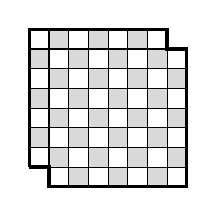
\begin{tikzpicture}[scale=.25]
\foreach \x in {0,2,...,6}{
	\foreach \y in {0,2,...,6}{
\draw[fill=white!85!black] (\x,\y) rectangle (\x+1, \y+1) rectangle (\x+2,\y+2);
}}
\draw (0,0) grid (8,8);
\draw[white, fill=white] (7,7) rectangle (8,8) (0,0) rectangle (1,1);
\draw[very thick] (0,1) -- (1,1) -- (1,0) -- (8,0) --(8,7) -- (7,7) -- (7,8) -- (0,8) -- (0,1);
\end{tikzpicture}
\end{center}

\begin{solution}
First notice that both removed squares have identical color. So their removal leaves us with $\frac{n}{2}$ squares of one color and $\frac{n-2}{2}$ squares of the other color. Since a domino always covers one black and one white squares, the remaining squares cannot be tiled.
\end{solution}


 
\end{questions}
\end{document}


